\section{Potek reševanja}
Pričel sem z vzpostavitvijo ogrodja, ki mi je omogočalo integracijo gibalnih enačb pri različnih parametrih. Najprej sem se uveril, da znam izračunati trajektorijo pri najbolj osnovnih začetnih pogojih
\[\left[x,y,u,v \right] = \left[1,0,0,1 \right].\]
Dobil sem spodnjo trajektorijo, ki ustreza krožni orbiti:

\begin{center}
     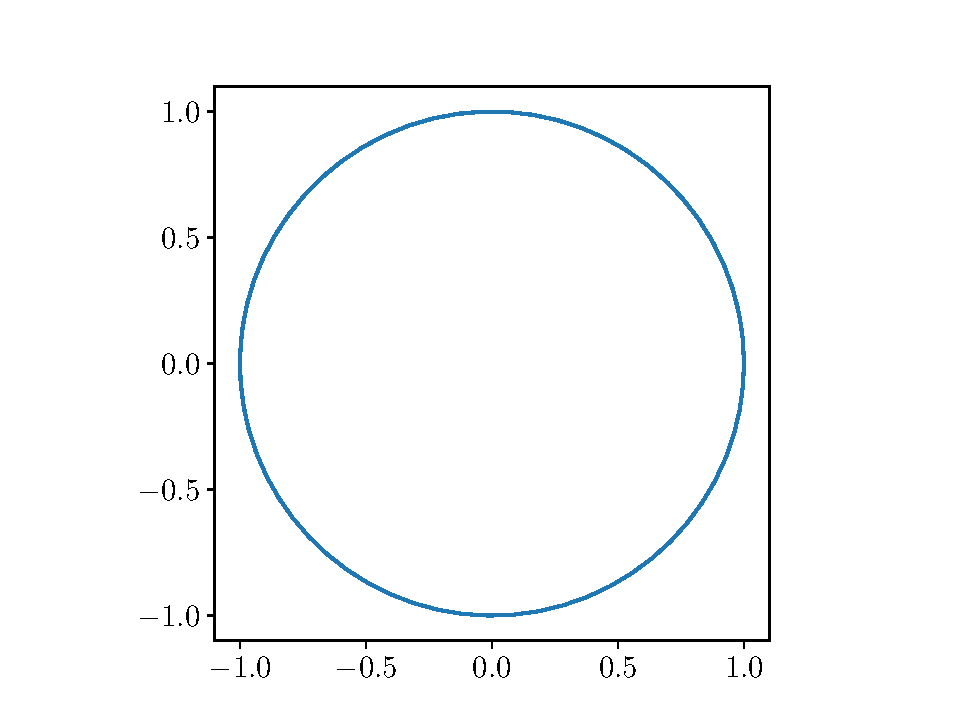
\includegraphics[width=0.5\textwidth]{0-simple-trajectory.pdf}
\end{center}

Naslednji korak je bila evalvacija konstantnosti invariantnih količin (\HH, \LL{} in $\vec{{A}}$) v odvisnosti od časovnega koraka. Najprej sem pogledal fluktuacije v \HH{}:

\begin{center}
     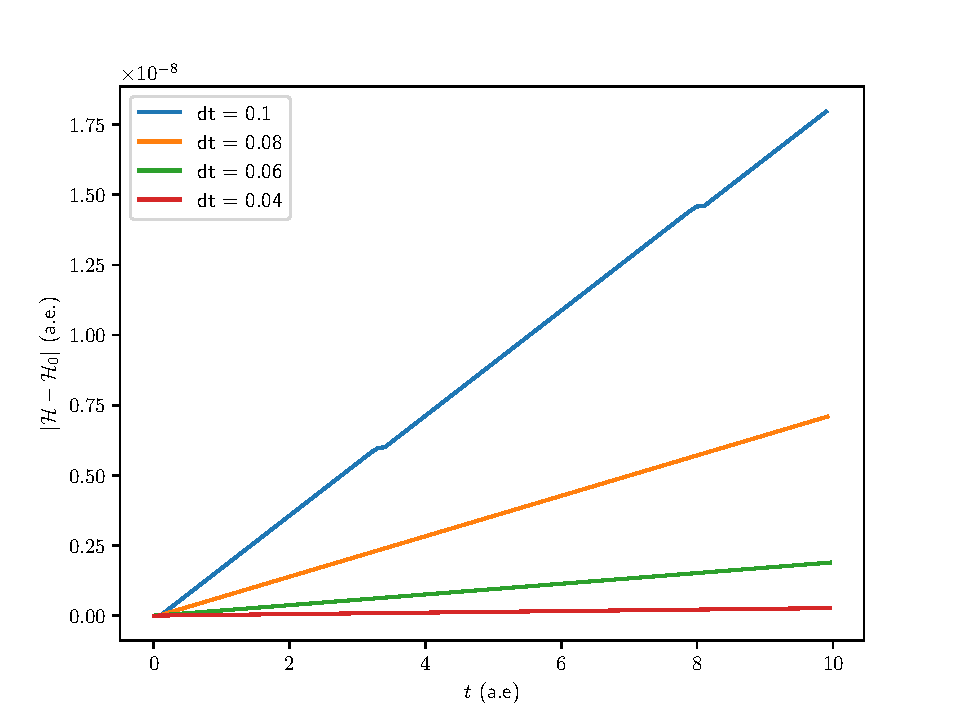
\includegraphics[width=0.7\textwidth]{1-H.pdf}
\end{center}

Nepresenetljivo z manjšim korakom fluktuacije Hamiltonove funkcije padajo. Bolje lahko to raziščem z opazovanjem standardnega odklona \HH{} v odvisnosti od koraka:

\begin{center}
     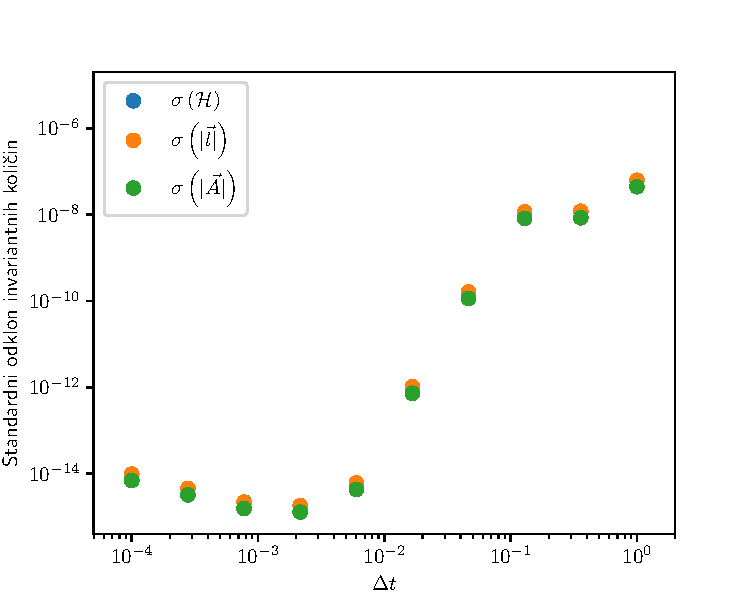
\includegraphics[width=0.7\textwidth]{1-stds.pdf}
\end{center}

Tu sem v obravnavo dodal še magnitudi \LL{} in $\vec{A}$. Vse invariantne količine se obnašajo enako; njihove fluktuacije lahko znižam z zmanjševanjem časovnega koraka, a le do neke točke, nakar pričnejo ponovno naraščati, kar pripišemo akumulaciji napak pri računanju s končno točnostjo.

\begin{samepage}
Z boljšim uvidom si poglejmo še trajektorije in pripadajoče Poincaréjeve preseke\footnote{Poincaréjeve preseke računam ob prehodu iz prvega v drugi kvadrant, na vodoravno os nanašam $y$, na navpično pa $v$. }, določene z linearno interpolacijo. Pričnem z začetnimi pogoji kot na začetku poročila, za primerjavo pa sem na isto sliko izrisal rezultate za dva časovna koraka. Na skali celotne trajektorije se razlika ne opazi, na Poincaréjevem preseku pa je precejšnja.

\begin{center}
     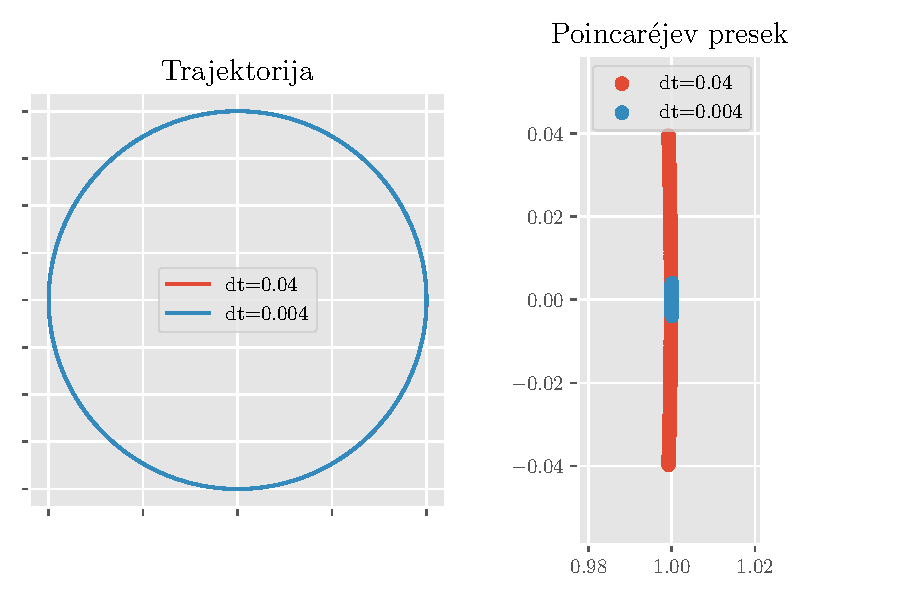
\includegraphics[width=0.7\textwidth]{1-poincare1.pdf}
\end{center}
\end{samepage}

 Ker me je zanimalo, kam se ``odpelje'' Poincaréjev presek za dolge čase integracije, sem z grobim korakim integriral dolg čas in dobil spodnjo sliko. 
\begin{center}
     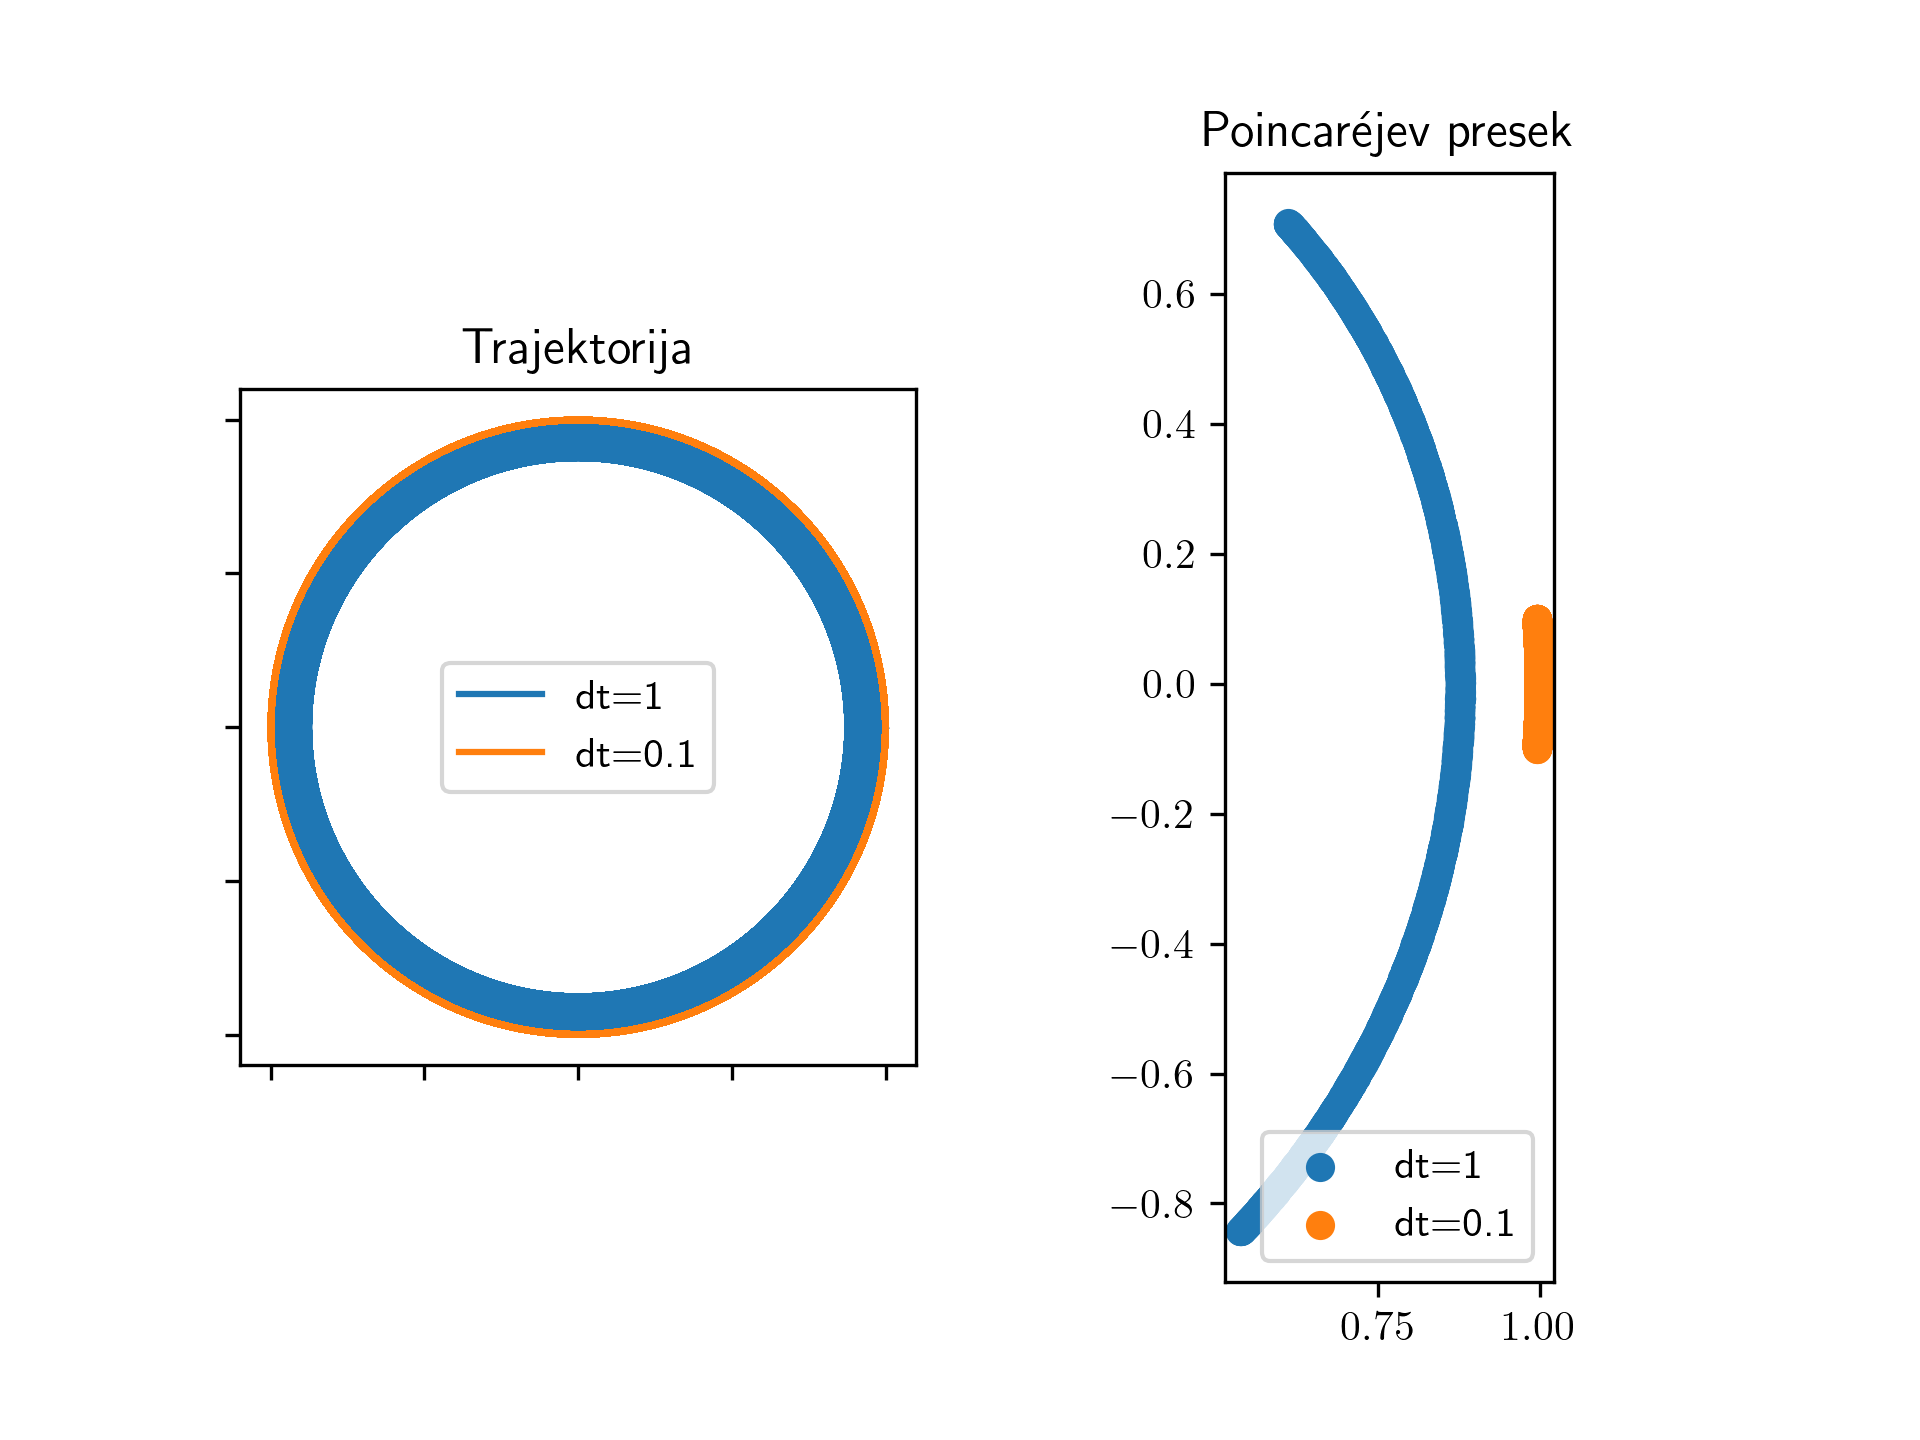
\includegraphics[width=0.7\textwidth]{1-poincare1-1.png}
\end{center}


Če si ogledamo splošna vezana stanja, opazimo še bolj divja obnašanja Poincaréjevega preseka, kjer se v faznem prostoru razmažejo tako krajevne količine kot tudi gibalne količine. Evidentno je, da naraščajoča eliptičnost orbite povzroči večjo razmazanost v Poincaréjevem preseku.
\begin{center}
     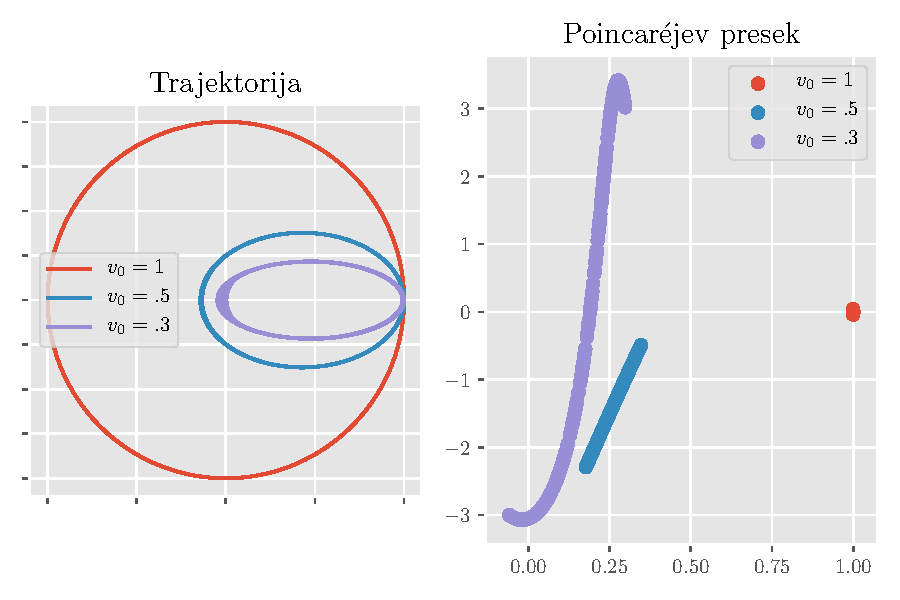
\includegraphics[width=0.7\textwidth]{1-poincare4.pdf}
\end{center}


Za raziskovanje točnosti obhodnega časa sem popravil interpolacijsko funkcijo za interpolacijo obhodnega časa (namesto prej uporabljenih krajevnih in hitrostnih koordinat). Pri različnih korakih sem gledal periodo in njen standardni odklon. Za preprosto kroženje velik časovni korak pomeni večje fluktuacije, vpliva na izmerjen obhodni čas pa ne zaznam:
\begin{center}
     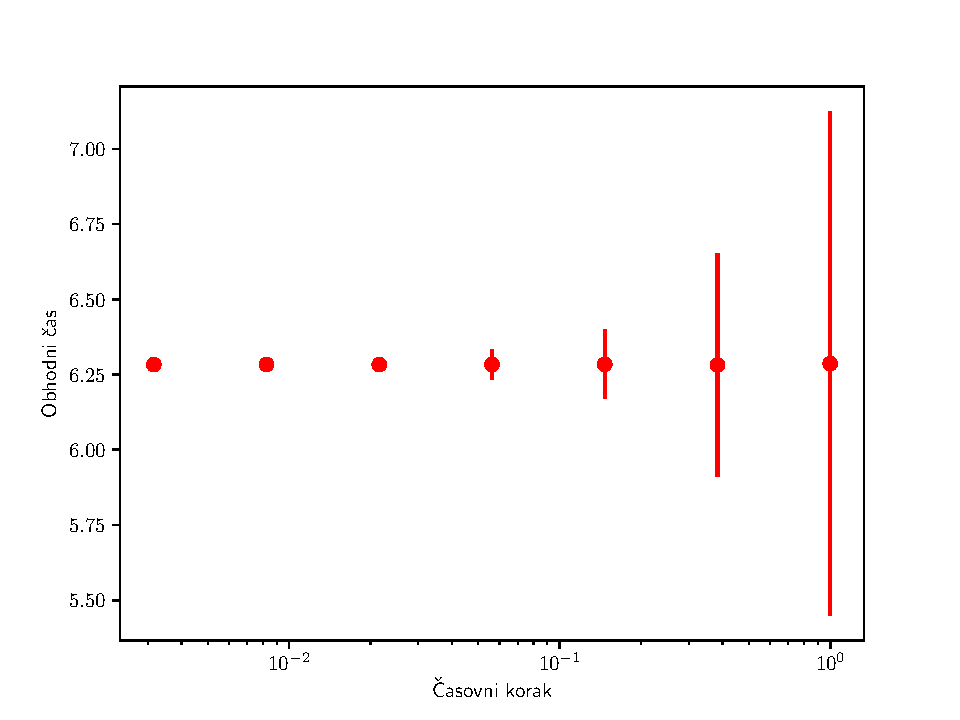
\includegraphics[width=0.7\textwidth]{1-periode.pdf}
\end{center}

Zgodba je krepko drugačna, če obdelavo ponovimo za močno eliptične orbite; tedaj z povečevanjem koraka ne povečamo le fluktuacij okrog prave vrednosti, marveč (vsaj z izbrano linearno interpolacijo) namerimo celo povečevanje obhodnega časa:
\begin{center}
     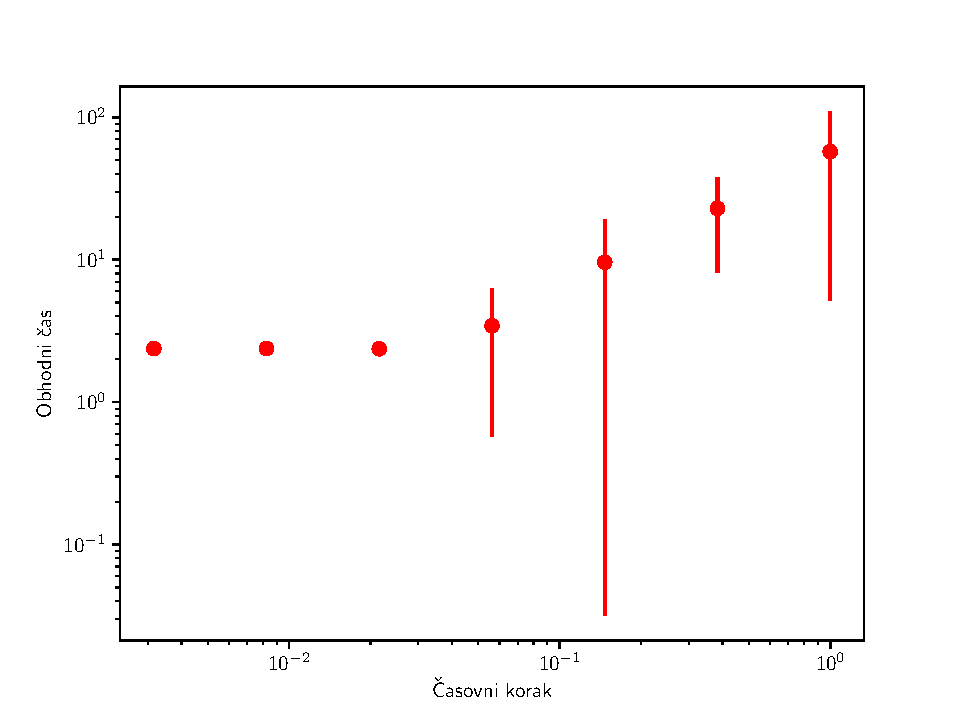
\includegraphics[width=0.7\textwidth]{1-periode_elipticno.pdf}
\end{center}

V nadaljevanju sem sonce nadomestil z dvema `polsolncema', ki sta krožila okrog skupnega težišča v krogu z radijem $R$. Privzamemo, da orbita planeta ne vpliva na gibanje solnc, druga uporabljena predpostavka pa je, da lahko fiksiram obodno hitrost dvozvezdja na 1, ker izvrednotenje fizikalno smiselne obodne hitrosti ne pripomore k pedagoški vrednosti naloge o ODE. Kot bi pričakovali, je obnašanje pogojeno z $R$: pri majhnih $R$ je orbita planeta podobna kroženju, ki smo ga videli v prvem delu poročila, ko pa $R$ raste, pa pričnemo videvati vse lepote kaotičnega gibanja treh teles. Za $R=0.1$ dobimo spodnjo trajektorijo in Poincaréjev presek:
\begin{center}
     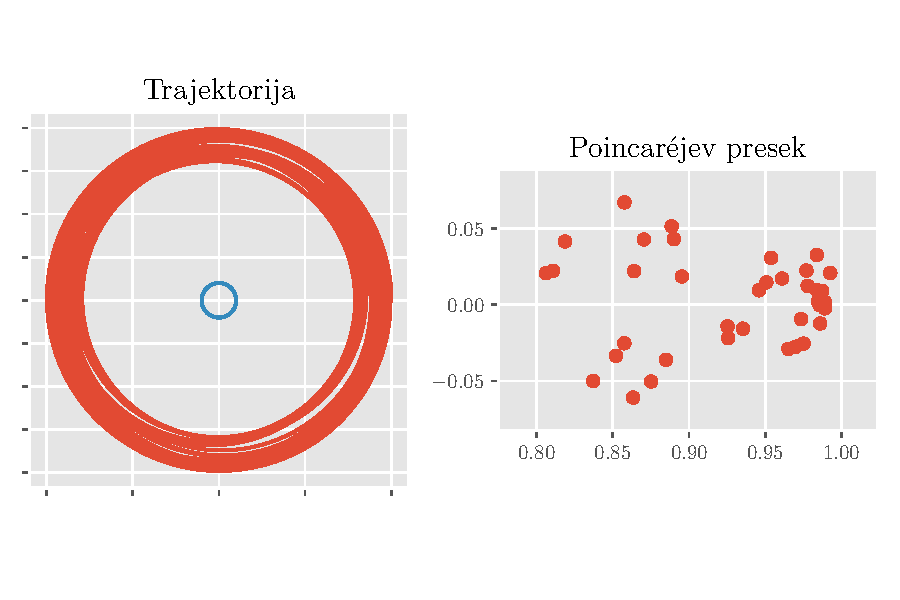
\includegraphics[width=0.7\textwidth]{2-small_R.pdf}
\end{center}
Ko povečamo $R$ na 0.5, postane gibanje bolj pestro:
\begin{center}
     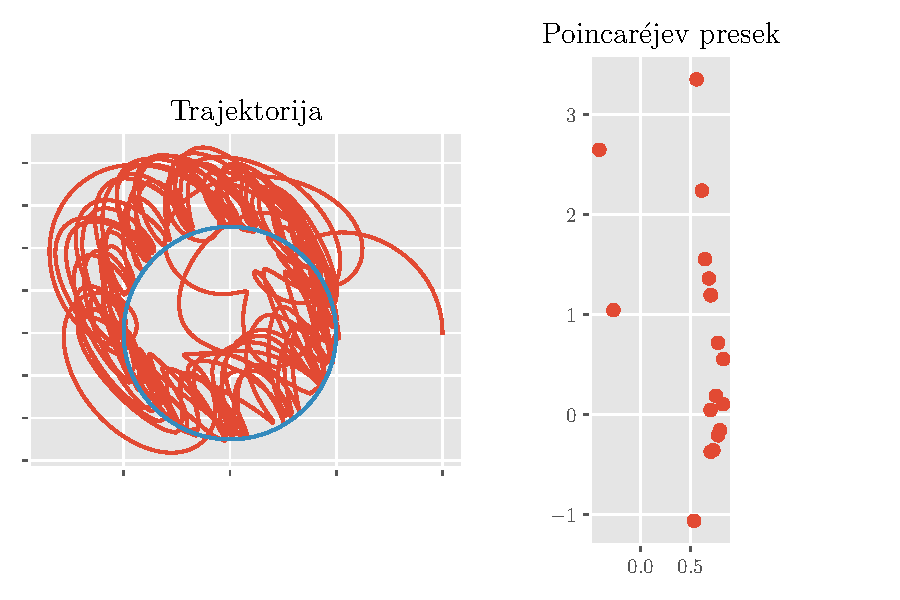
\includegraphics[width=0.7\textwidth]{2-big_R.pdf}
\end{center}
Ko pa $R$ povečamo na 1.2, lahko `ujamemo' planet v orbito enega od solnc, zaradi česar postane gibanje bolj regularno, a z nekesortnimi Ptolemaičnimi epicikli.
\begin{center}
     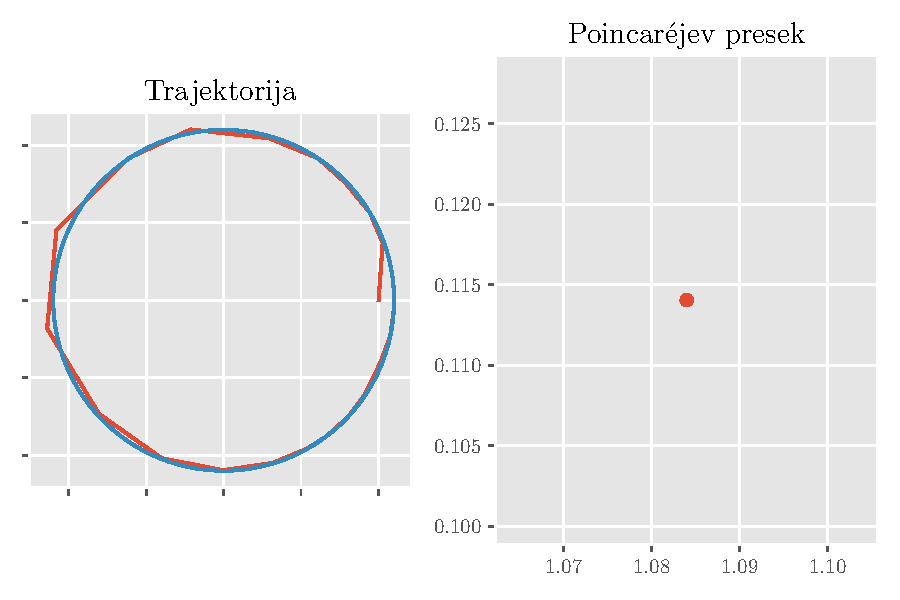
\includegraphics[width=0.7\textwidth]{2-bigbig_R.pdf}
\end{center}

Pri tretjem delu sem popravil diferencialne enačbe, ki pogojujejo gibanje dvozvezdja, kot zahteva naloga. S standardnimi začetnimi pogoji sem pognal integracijo in dobil spodnjo trajektorijo in Poincaréjev presek:
\begin{center}
     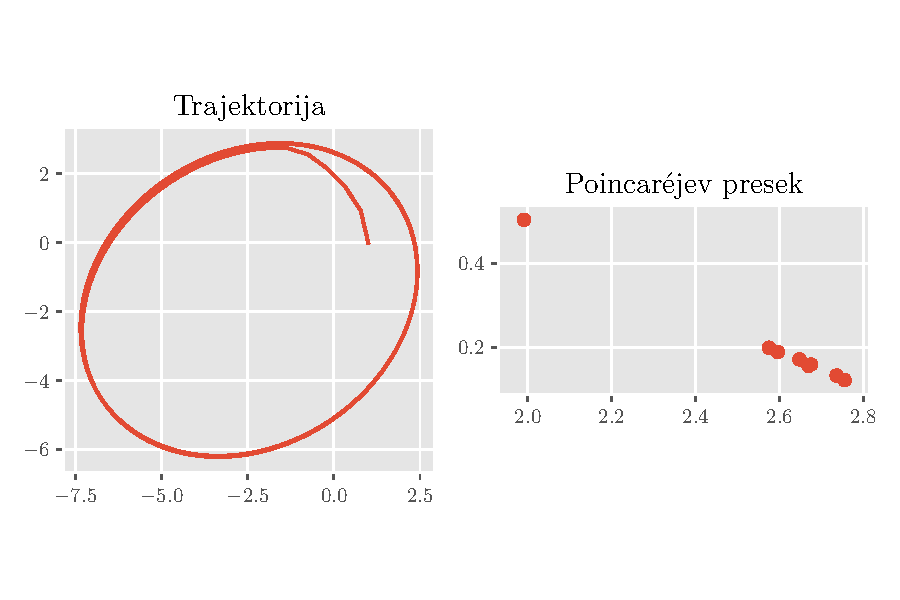
\includegraphics[width=0.7\textwidth]{3-trajektorija.pdf}
\end{center}
Ko sem ugotovil, da naloga zahteva, da simulacijo prekinemo, ko je gibajoče solnce za enako razdaljo oddaljeno od začetne točke, sem dodal še vez za maksimalen čas integracije. Za raziskovanje usode planeta potrebujemo primerno metriko. Eno smo že uvedli, to je Hamiltonova funkcija \HH{}; če je ob koncu integracije nenegativna, planet ni gravitacijsko vezan na dvozvezdje. V nasprotnem primeru lahko pogledamo vezavni energiji $E_{1}$ in $E_2$, kjer indeksa označujeta prvo ali drugo solnce. Privzamemo, da bo planet ostal vezan na solnce, s katerim je ob koncu simulacije močneje vezan. Zaradi spreminjajoče faze sem pripravil rotacijsko matriko, s katero sem rotiral krajevne in hitrostne vektorje, v diferencialne enačbe pa sem dodal tudi enačbi za premo gibanje mimobežnega solnca. Rezultat reševanja je bila matrika, katere stolpci so bili časovni poteki količin $\left( x,y,u,v,x_2,y_2,\mathcal{H}, E_1, E_2 \right)$, čeprav bi dejansko potreboval samo zadnjo vrstico. Najprej sem se malo poigral z različnimi začetnimi parametri in našel nekaj zanimivih režimov, tudi take, kjer mimobežno solnce iztiri krožeč planet.

\begin{center}
     \includegraphics[width=0.7\textwidth]{3-trajektorija2.pdf}
\end{center}
\begin{center}
     \includegraphics[width=0.7\textwidth]{3-trajektorija3.pdf}
\end{center}
\begin{center}
     \includegraphics[width=0.7\textwidth]{3-trajektorija4.pdf}
\end{center}
\begin{center}
     \includegraphics[width=0.7\textwidth]{3-trajektorija5.pdf}
\end{center}
Za iskanje obnašanja sem integracijo pognal na mreži različnih faz in začetnih hitrosti, nato pa ovrednotil usodo planeta v vsaki točki. Če je planet po srečanju nevezan, označim to z vrednostjo 0, sicer pa z vrednostjo 1 ali 2, če je planet vezan na prvo ali drugo solnce. Opazim, da pri najbolj ekscentričnih orbitah evaluacija traja najdlje; to pojasnimo z dolgim časom trajanja simulacije, ki je vezan na čas, ki ga mimobežno solnce potrebuje, da se premakne do svoje končne točke. Z relativno grobo mrežo 8x8 dobim spodnjo sliko:
\begin{center}
     \includegraphics[width=0.7\textwidth]{3-gridsearch-imshow.pdf}
\end{center}
Tu rumena barva predstavlja vezano stanje z drugim (mimobežnim) solncem, smaragdna vezano stanje s prvim (mirujočim) solncem, in temno modra nevezano stanje. Če smo sitni in povečamo resolucijo mreže na 24x24, se prikažejo še dodatni detajli portreta faznega prostora:
\begin{center}
     \includegraphics[width=0.7\textwidth]{3-gridsearch-imshow2.pdf}
\end{center}
Kot izgleda, prav najzahtevnejša področja okrog $v_0 = 0$ skrivajo pestro dinamiko. Če se odpovemo ekvidistančnem vzorčenju v težavnem področju okrog ničle v hitrostni koordinati, lahko najdemo tudi druge regije z nepričakovanimi usodami za krožečo zemljo. V malenkost drugačni barvni shemi jih prikazujem spodaj. Fazna resolucija znaša 50 točk, hitrostna pa 100.
\begin{center}
     \includegraphics[width=0.9\textwidth]{3-gridsearch-contourf.pdf}
\end{center}
Če resolucijo povečamo na 130x260 točk, dobimo:
\begin{center}
     \includegraphics[width=0.9\textwidth]{3-gridsearch-contourf_3.pdf}
\end{center}